% Rapport final — Projet « Apprentissage non supervisé » — compilation : xelatex rapport.tex (x2)
\documentclass[11pt,a4paper]{article}
\usepackage{fontspec}
\usepackage{polyglossia}
\setmainlanguage{french}
\usepackage{amsmath,amssymb}
\usepackage[margin=2.2cm]{geometry}
\usepackage{graphicx,booktabs,tabularx,multirow,float,caption,enumitem,xcolor,fancyhdr,titlesec,microtype}
\usepackage[hidelinks]{hyperref}
\graphicspath{{../reports/figures/}}

\definecolor{bleu}{HTML}{1F3A5F}
\definecolor{s1}{HTML}{7F8C8D}\definecolor{s2}{HTML}{2E86C1}\definecolor{s3}{HTML}{C0392B}\definecolor{s4}{HTML}{E67E22}
\titleformat{\section}{\Large\bfseries\color{bleu}}{\thesection}{.6em}{}
\titleformat{\subsection}{\large\bfseries\color{bleu}}{\thesubsection}{.6em}{}
\captionsetup{font=small,labelfont=bf}
\setlist{itemsep=2pt,topsep=4pt}
\pagestyle{fancy}\fancyhf{}
\lhead{\small Segmentation de clientèle bancaire}\rhead{\small Master BDA/IA — Apprentissage non supervisé}
\cfoot{\thepage}
\setlength{\parskip}{4pt}

\begin{document}

\begin{titlepage}
\centering
\vspace*{2cm}
{\large Université Numérique Cheikh Hamidou Kane — Master Big Data Analytics / IA\par}
\vspace{.3cm}
{\large Module « Apprentissage non supervisé » — Projet final\par}
\vspace{2.5cm}
{\color{bleu}\rule{\linewidth}{1pt}\par\vspace{.4cm}
{\Huge\bfseries Segmentation de clientèle bancaire\\[.2cm] par apprentissage non supervisé\par}
\vspace{.4cm}\rule{\linewidth}{1pt}\par}
\vspace{1cm}
{\large Jeu de données \textit{Bank Marketing} (UCI) — 41\,188 clients, 20 variables\par}
\vspace{3cm}
{\Large Papa Alassane SECK\par}
\vspace{.3cm}
{\large Octobre 2026\par}
\vfill
\begin{minipage}{.85\linewidth}\small
\textbf{Résumé.} Nous segmentons les clients d'une banque portugaise ciblés par des campagnes de télémarketing à partir de données mixtes, sans utiliser la variable de souscription. Après préparation (exclusion justifiée de \texttt{duration}, encodages, standardisation, PCA/t-SNE/UMAP), nous comparons cinq distances et sept familles d'algorithmes (K-means, K-medoids/Gower, K-prototypes, GMM, CAH à quatre liens, DBSCAN). La validation interne, externe et de stabilité conduit à retenir une \textbf{classification mixte (CAH Ward + consolidation K-means) à 4 segments} (silhouette 0,192, Davies-Bouldin 1,69). Les taux de souscription y varient de 4,9\,\% à 42,5\,\% : trois segments réunissant 35\,\% des clients concentrent 72\,\% des souscripteurs. Quatre recommandations marketing, une application Streamlit et quatre extensions (anomalies, sélection de variables, RFM) complètent l'étude.
\end{minipage}
\end{titlepage}

\tableofcontents
\newpage

%=====================================================================
\section{Introduction}
Une banque souhaite mieux connaître ses clients pour cibler ses campagnes de marketing téléphonique visant la souscription d'un \textbf{dépôt à terme}. Aucune segmentation n'existe : il s'agit de \emph{découvrir} des groupes homogènes de clients à partir de variables numériques et catégorielles, puis d'en évaluer la qualité et l'utilité métier.

Le problème est non supervisé : la variable \texttt{y} (souscription oui/non) n'est \textbf{jamais} utilisée pour l'apprentissage. Elle sert uniquement de vérité terrain pour les indices externes (ARI, NMI, V-mesure) et, \emph{a posteriori}, pour mesurer le taux de souscription des segments.

Le projet mobilise les quatre chapitres du cours : préparation des données (§\ref{sec:prep}), mesures de dissimilarité (§\ref{sec:dist}), méthodes de clustering (§\ref{sec:part}–\ref{sec:hier}) et validation (§\ref{sec:valid}). L'interprétation et les recommandations font l'objet du §\ref{sec:interp}, les extensions du §\ref{sec:bonus}. Le code (7 notebooks exécutables, module de prétraitement réutilisable, application Streamlit) est fourni avec le rapport ; la graine aléatoire est fixée à 42.

%=====================================================================
\section{Données et préparation}\label{sec:prep}
\subsection{Description de la matrice de données}
Le fichier \texttt{bank-additional-full.csv} contient \textbf{41\,188 individus × 21 variables} (mai 2008 – novembre 2010). On distingue :
\begin{itemize}
\item \textbf{continues} : \texttt{age}, \texttt{duration}, cinq indicateurs macro-économiques (\texttt{emp.var.rate}, \texttt{cons.price.idx}, \texttt{cons.conf.idx}, \texttt{euribor3m}, \texttt{nr.employed}) ;
\item \textbf{discrètes} : \texttt{campaign}, \texttt{pdays} (999 = jamais contacté), \texttt{previous} ;
\item \textbf{nominales} : \texttt{job} (12 modalités), \texttt{marital}, \texttt{poutcome}, \texttt{month}, \texttt{day\_of\_week} ;
\item \textbf{ordinale} : \texttt{education} (de \textit{illiterate} à \textit{university.degree}) ;
\item \textbf{binaires} : \texttt{default}, \texttt{housing}, \texttt{loan} (avec modalité \textit{unknown}), \texttt{contact} ; cible \texttt{y} (11,3\,\% de « yes »).
\end{itemize}

\subsection{Nettoyage}
Le tableau~\ref{tab:clean} résume les décisions. Il n'y a pas de \texttt{NaN} au sens strict : les manquants sont codés \textit{unknown}.

\begin{table}[H]\centering\small
\begin{tabularx}{\linewidth}{lXX}
\toprule
\textbf{Problème} & \textbf{Décision} & \textbf{Justification}\\\midrule
12 doublons exacts & suppression (41\,176 clients) & aucune information ajoutée\\
\texttt{job} (330), \texttt{marital} (80) \textit{unknown} & imputation par le mode & < 1\,\% des lignes\\
\texttt{education} (1\,731 \textit{unknown}) & mode \emph{au sein du métier} & 4,2\,\% ; l'éducation dépend du métier\\
\texttt{housing}/\texttt{loan} (990, mêmes lignes) & imputation par le mode & 2,4\,\%\\
\texttt{default} : 21\,\% \textit{unknown}, 3 « yes » & binaire \texttt{default\_flag} = « non déclaré sans défaut » & \textit{unknown} est informatif\\
\texttt{campaign} (max 56, 5,8\,\% aberrants IQR) & écrêtage au 99\textsuperscript{e} centile (14) puis $\log(1+x)$ & limite l'influence de quelques clients\\
\texttt{age} > 69 ans (1,1\,\% aberrants IQR) & conservés & retraités réels, segment pertinent\\
\bottomrule
\end{tabularx}
\caption{Décisions de nettoyage.}\label{tab:clean}
\end{table}

\subsection{Analyse exploratoire et choix des variables}
\begin{figure}[H]\centering
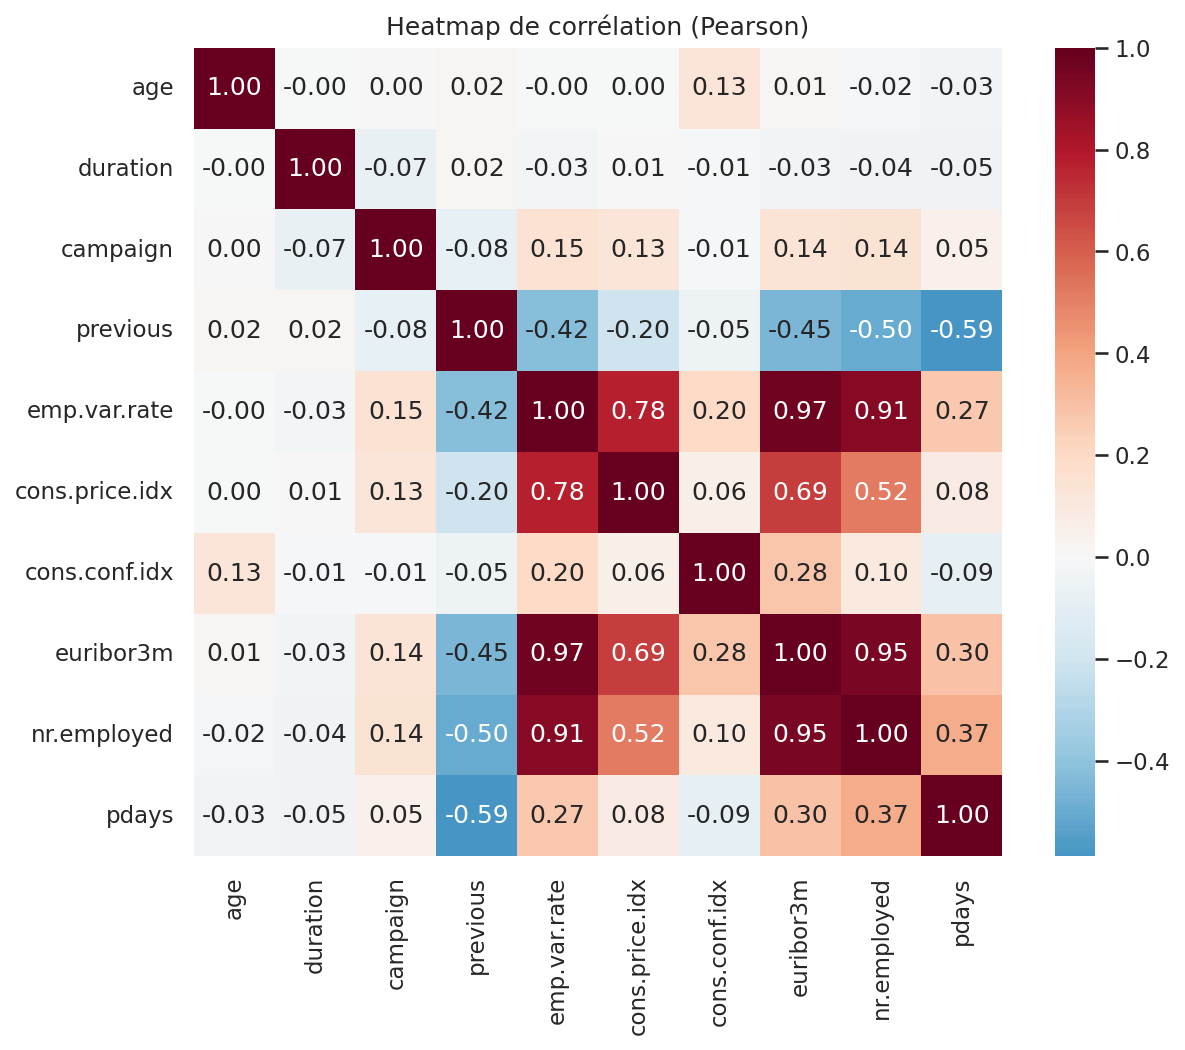
\includegraphics[width=.62\linewidth]{j1_heatmap_corr.png}
\caption{Corrélations de Pearson : les indicateurs macro-économiques sont quasi colinéaires.}\label{fig:corr}
\end{figure}

L'EDA (histogrammes, diagrammes en barres, nuages de points, figure~\ref{fig:corr}) conduit à quatre décisions structurantes :
\begin{enumerate}
\item \textbf{\texttt{duration} est exclue} : la durée du dernier appel n'est connue qu'\emph{après} l'appel ; l'utiliser pour segmenter des clients avant une campagne serait une fuite d'information.
\item \texttt{emp.var.rate}, \texttt{euribor3m} et \texttt{nr.employed} sont corrélés à 0,91–0,97 et \texttt{cons.price.idx} à environ 0,7. On garde \texttt{euribor3m} (cycle des taux) et \texttt{cons.conf.idx} (confiance des ménages, peu corrélée) pour ne pas compter quatre fois la même information.
\item \texttt{month} et \texttt{day\_of\_week} décrivent le calendrier d'appel, pas le client : exclues.
\item \texttt{pdays} vaut 999 dans 96\,\% des cas et duplique \texttt{previous}/\texttt{poutcome} : exclue.
\end{enumerate}
On retient \textbf{13 variables} : 6 numériques/ordinales (\texttt{age}, \texttt{campaign\_log}, \texttt{previous}, \texttt{euribor3m}, \texttt{cons.conf.idx}, \texttt{education\_level}), 4 binaires (\texttt{housing}, \texttt{loan}, \texttt{default\_flag}, \texttt{contact\_cellular}) et 3 nominales (\texttt{job}, \texttt{marital}, \texttt{poutcome}).

\subsection{Deux représentations et échantillon de travail}
\begin{itemize}
\item \textbf{(a)} numériques standardisées $z=(x-\mu)/\sigma$, binaires 0/1, nominales en \emph{one-hot} : 27 colonnes ; utilisée par K-means, GMM, CAH euclidienne, DBSCAN.
\item \textbf{(b)} données mixtes brutes (numériques dans leur unité, qualitatives en modalités) : utilisée par Gower, K-medoids et K-prototypes.
\end{itemize}
Les méthodes à matrice de distances étant en $O(n^2)$, toutes les comparaisons se font sur un \textbf{échantillon aléatoire stratifié de 4\,000 clients} (11,28\,\% de « yes » contre 11,27\,\% dans la population). Le modèle final est ensuite appliqué à toute la population. Toute la logique est encapsulée dans \texttt{src/preprocessing.py} (\texttt{preprocess()}, \texttt{transform\_new\_client()}).

\subsection{Réduction de dimension}
La PCA sur (a) montre une variance diffuse : PC1 = 21,0\,\%, PC2 = 15,5\,\%. Il faut \textbf{7 composantes pour 80\,\%} et 12 pour 90\,\%. PC1 est portée par le contexte de taux et l'historique de contact (\texttt{euribor3m}, \texttt{previous}), PC2 par le cycle de vie (âge, éducation). Les méthodes non linéaires révèlent une structure en \textbf{îlots} invisible en PCA (figure~\ref{fig:emb}).

\begin{figure}[H]\centering
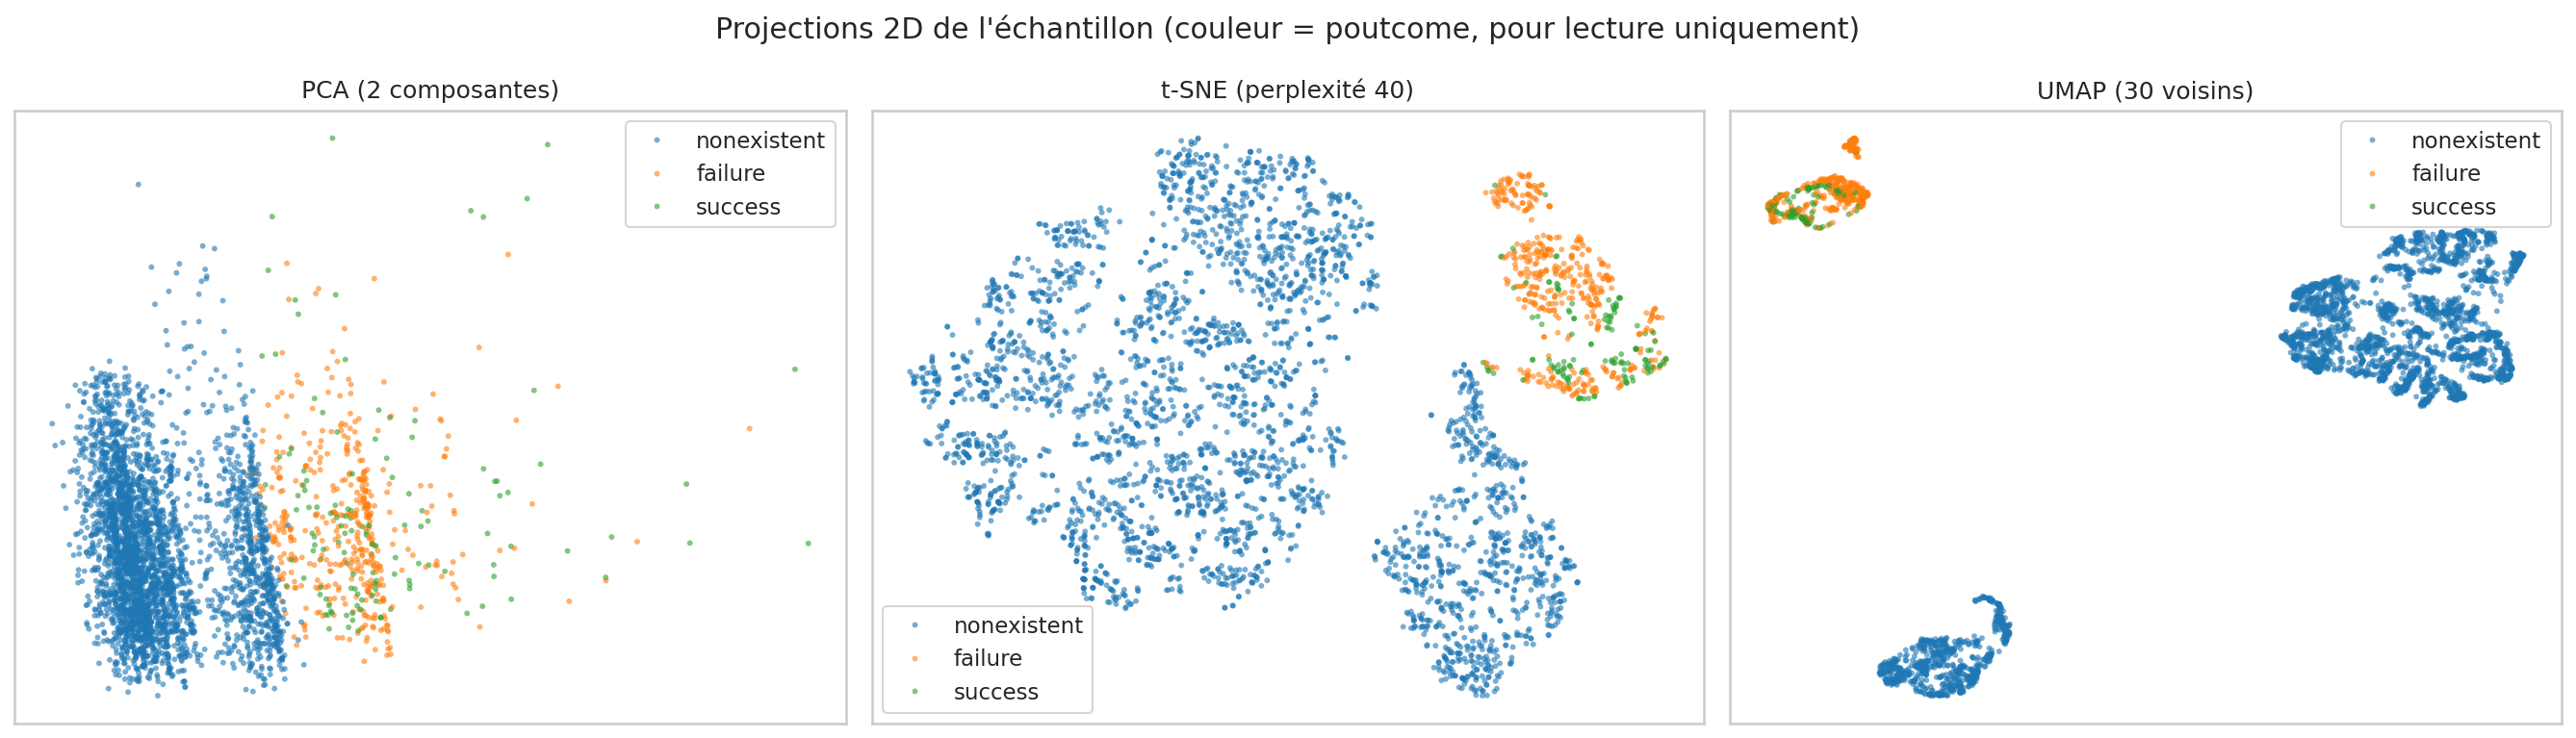
\includegraphics[width=\linewidth]{j1_pca_tsne_umap.png}
\caption{PCA, t-SNE et UMAP sur l'échantillon (couleur : \texttt{poutcome}, pour lecture seulement).}\label{fig:emb}
\end{figure}

%=====================================================================
\section{Mesures de dissimilarité}\label{sec:dist}
Cinq matrices $4\,000\times4\,000$ ont été calculées :
\begin{itemize}
\item \textbf{euclidienne} et \textbf{Manhattan} sur (a) ;
\item \textbf{Gower} sur (b) : $d(x,y)=\frac1p\sum_j d_j$, avec $d_j=|x_j-y_j|/R_j$ pour une variable numérique et $d_j=\mathbb 1[x_j\neq y_j]$ pour une variable qualitative ;
\item \textbf{Hamming} et \textbf{Jaccard} sur le bloc binaire de 21 colonnes.
\end{itemize}

\begin{table}[H]\centering\small
\begin{tabular}{lccccc}\toprule
 & Euclid. & Manhattan & Gower & Hamming & Jaccard\\\midrule
Euclidienne & 1 & 0,93 & 0,71 & 0,48 & 0,44\\
Manhattan & & 1 & 0,86 & 0,70 & 0,65\\
Gower & & & 1 & 0,86 & 0,80\\
Hamming & & & & 1 & 0,94\\\bottomrule
\end{tabular}
\caption{Corrélations de Spearman entre dissimilarités (200\,000 paires).}\label{tab:rho}
\end{table}

Euclidienne et Manhattan ordonnent les paires de façon proche. Gower est plus liée à Manhattan, dont elle est une moyenne normalisée, et aux mesures binaires, car 7 de ses 13 variables sont qualitatives. Elle diffère de l'euclidienne sur (a), où une variable à $m$ modalités pèse plus lourd (un changement de métier modifie deux indicatrices). Jaccard ignore les co-absences 0–0, ce qui est pertinent pour des indicatrices \emph{one-hot} majoritairement nulles.

\paragraph{Effet de la standardisation.} Sans standardisation, \texttt{age} représente \textbf{80\,\%} de la distance euclidienne au carré et \texttt{cons.conf.idx} 15\,\%. \texttt{euribor3m}, \texttt{previous} et \texttt{campaign\_log} pèsent alors moins de 3\,\%. La corrélation de rang entre distances brute et standardisée n'est que de 0,55, et seuls \textbf{32\,\%} des 10 plus proches voisins sont conservés. Après z-score, chaque variable contribue à environ 16,7\,\%. La standardisation est donc indispensable pour toute méthode euclidienne ; Gower obtient un effet équivalent par l'étendue $R_j$.

%=====================================================================
\section{Méthodes de partitionnement}\label{sec:part}
\begin{itemize}
\item \textbf{K-means} (sur (a), population complète) : le coude de l'inertie (distance maximale à la corde) donne \textbf{k = 5}.
\item \textbf{K-medoids} (PAM, initialisation k-medoids++, sur Gower) : le coût décroît sans coude marqué et la silhouette Gower est maximale à \textbf{k = 3} (0,158). Les médoïdes sont de vrais clients.
\item \textbf{K-prototypes} (coût de Huang, numériques standardisées, $\gamma = 0{,}5$) : coude à \textbf{k = 5}.
\item \textbf{GMM} dans l'espace PCA à 80\,\% : un GMM à covariance pleine sur 27 colonnes majoritairement binaires serait dégénéré. Le BIC et l'AIC décroissent jusqu'à $k=10$ pour les quatre types de covariance, car les variables discrètes violent l'hypothèse gaussienne. On prend donc le coude du BIC, \textbf{k = 6}.
\end{itemize}

\begin{figure}[H]\centering
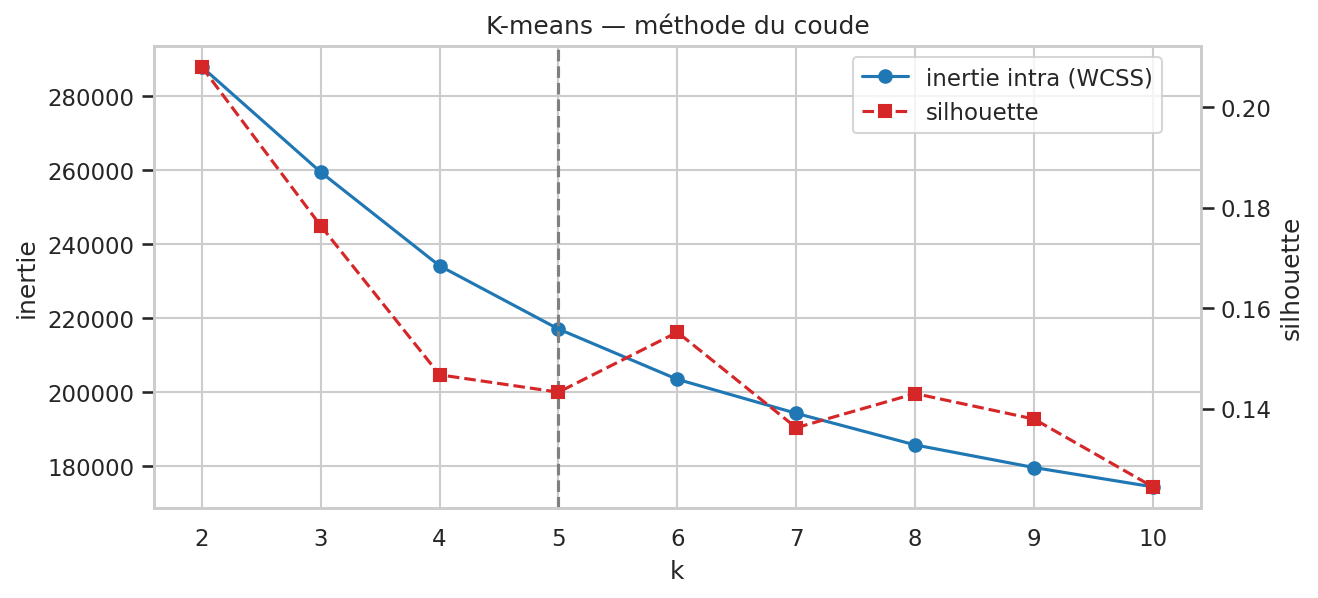
\includegraphics[width=.49\linewidth]{j2_kmeans_coude.png}\hfill
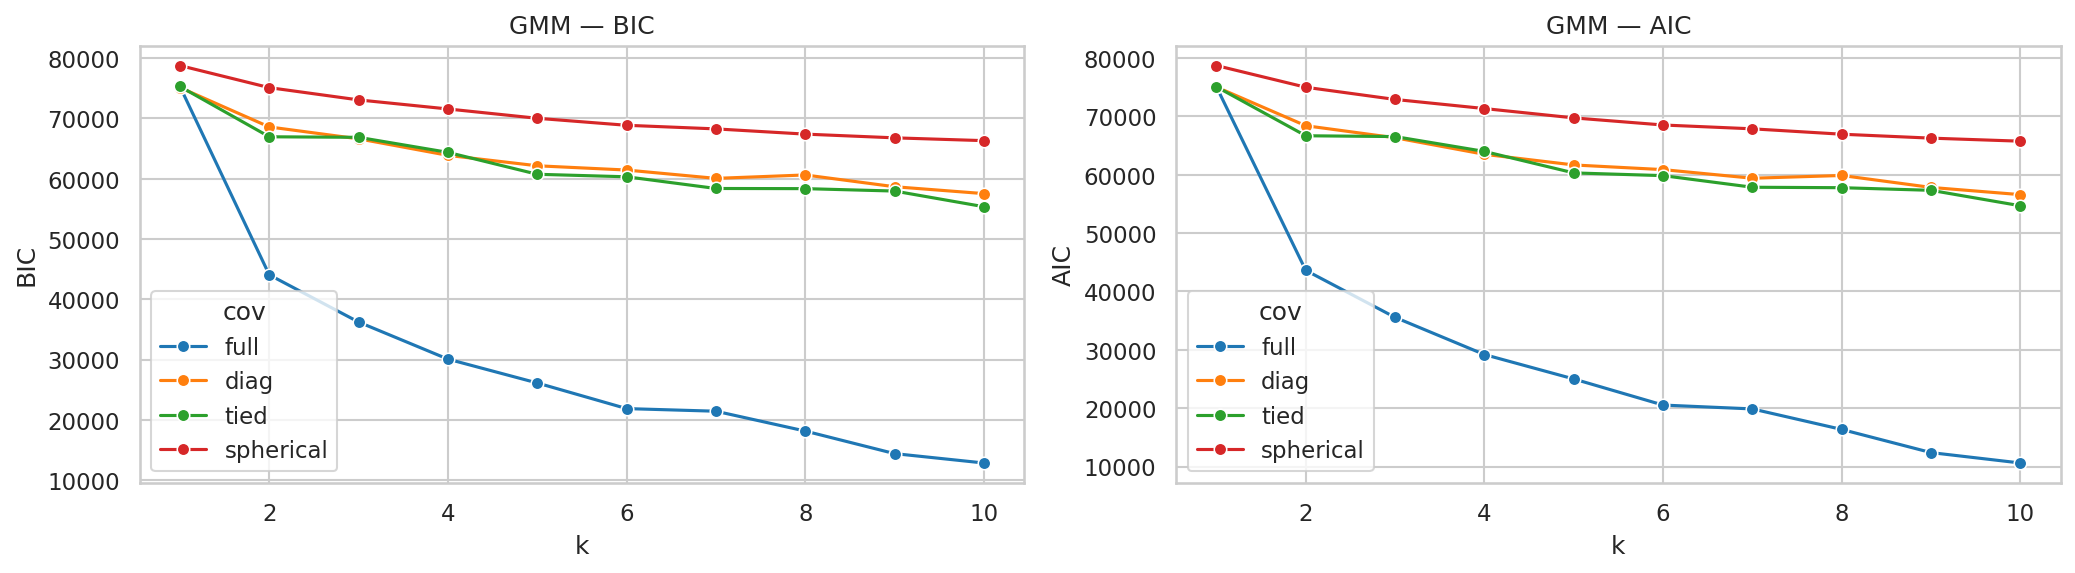
\includegraphics[width=.49\linewidth]{j2_gmm_bic_aic.png}
\caption{Méthode du coude pour K-means (gauche) ; critères BIC/AIC du GMM (droite, extrait).}
\end{figure}

\begin{table}[H]\centering\small
\begin{tabular}{lllcccc}\toprule
Méthode & Représentation & Distance & $k$ & Silh. (a) & DB (a) & Silh. native\\\midrule
K-means & (a) & euclidienne & 5 & 0,142 & 1,85 & 0,142\\
K-medoids & (b) & Gower & 3 & 0,059 & 2,89 & 0,158\\
K-prototypes & (b) & euclid. + $\gamma$·désaccord & 5 & 0,139 & 1,88 & 0,102\\
GMM (full) & PCA 80\,\% & probabiliste & 6 & 0,047 & 2,79 & —\\\bottomrule
\end{tabular}
\caption{Tableau comparatif du Jour 2 (indices calculés dans l'espace commun (a)).}\label{tab:j2}
\end{table}

K-means et K-prototypes dominent dans l'espace commun. K-medoids/Gower a la meilleure silhouette \emph{native} mais une mauvaise silhouette vue depuis (a) : les deux géométries ne racontent pas la même histoire, d'où l'importance du choix de la distance.

%=====================================================================
\section{Clustering hiérarchique et par densité}\label{sec:hier}
\subsection{Classification ascendante hiérarchique}
Quatre liens ont été testés en euclidienne (single, complete, average, Ward) et trois sur Gower.

\begin{figure}[H]\centering
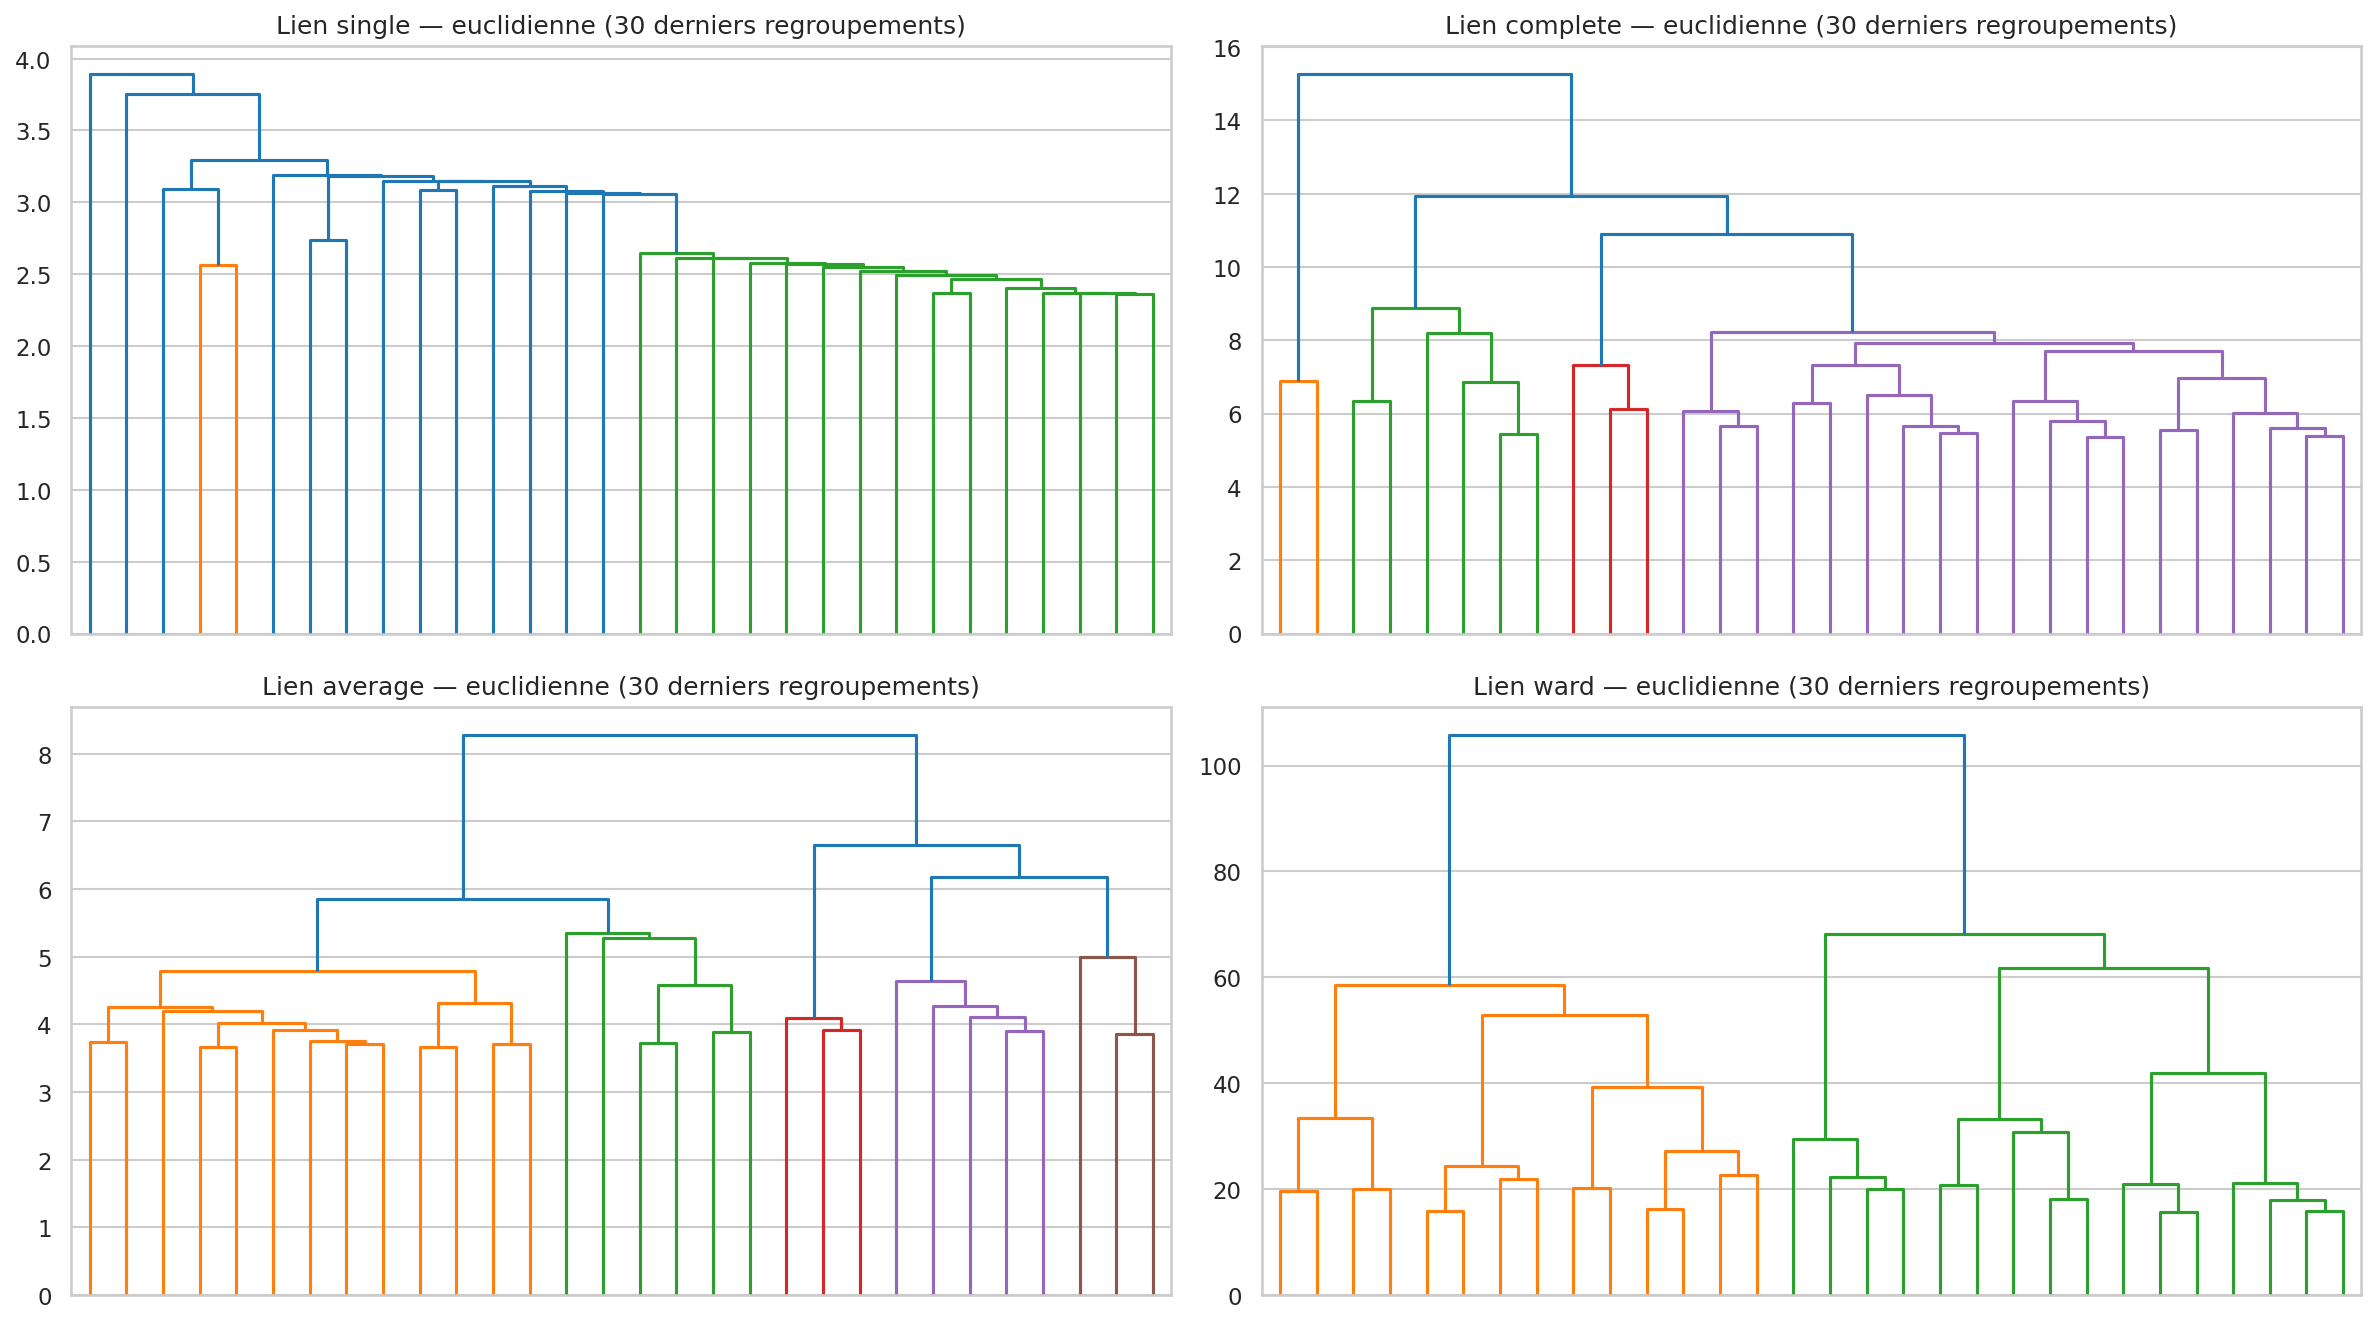
\includegraphics[width=.9\linewidth]{j3_dendrogrammes.png}
\caption{Dendrogrammes tronqués (30 derniers regroupements) pour les quatre liens.}
\end{figure}

\begin{itemize}
\item \textbf{Single} : silhouette la plus haute (0,68 à $k=2$) mais trompeuse. Le plus gros cluster regroupe 99,6 à 100\,\% des clients : c'est l'\emph{effet de chaîne}.
\item \textbf{Average / complete} : meilleure fidélité aux distances (corrélation cophénétique 0,78 et 0,74), mais un groupe dominant (> 95\,\% jusqu'à $k=7$). Ces liens isolent surtout des atypiques.
\item \textbf{Ward} : cophénétique plus faible (0,53), mais des groupes de tailles comparables. Le plus grand saut de hauteur suggère 5 groupes et la silhouette, pour $k\geq3$, culmine à \textbf{k = 4} (0,189 ; tailles 2\,616 / 603 / 325 / 456).
\end{itemize}

\subsection{DBSCAN}
\texttt{min\_samples} ($e^*$) est fixé, puis $\varepsilon$ ($d^*$) est lu au coude du graphique des $e^*$-distances triées (figure~\ref{fig:db}).
\begin{itemize}
\item Sur UMAP avec $e^*=10$ (règle $2\times$dim), $\varepsilon^*=0{,}23$ produit 17 micro-clusters.
\item Avec $e^*=50$, $\varepsilon^*=0{,}52$ donne \textbf{6 clusters, 3\,579 points cœur, 410 de bordure et 11 de bruit}.
\item La sensibilité est forte : avec $\varepsilon\times0{,}75$ on obtient 20 clusters et 314 bruits.
\item En PCA 7D, la densité est plus diffuse (3 clusters, 4\,\% de bruit).
\end{itemize}
Les clusters obtenus croisent période de taux (élevés ou bas) et historique de contact.

\begin{figure}[H]\centering
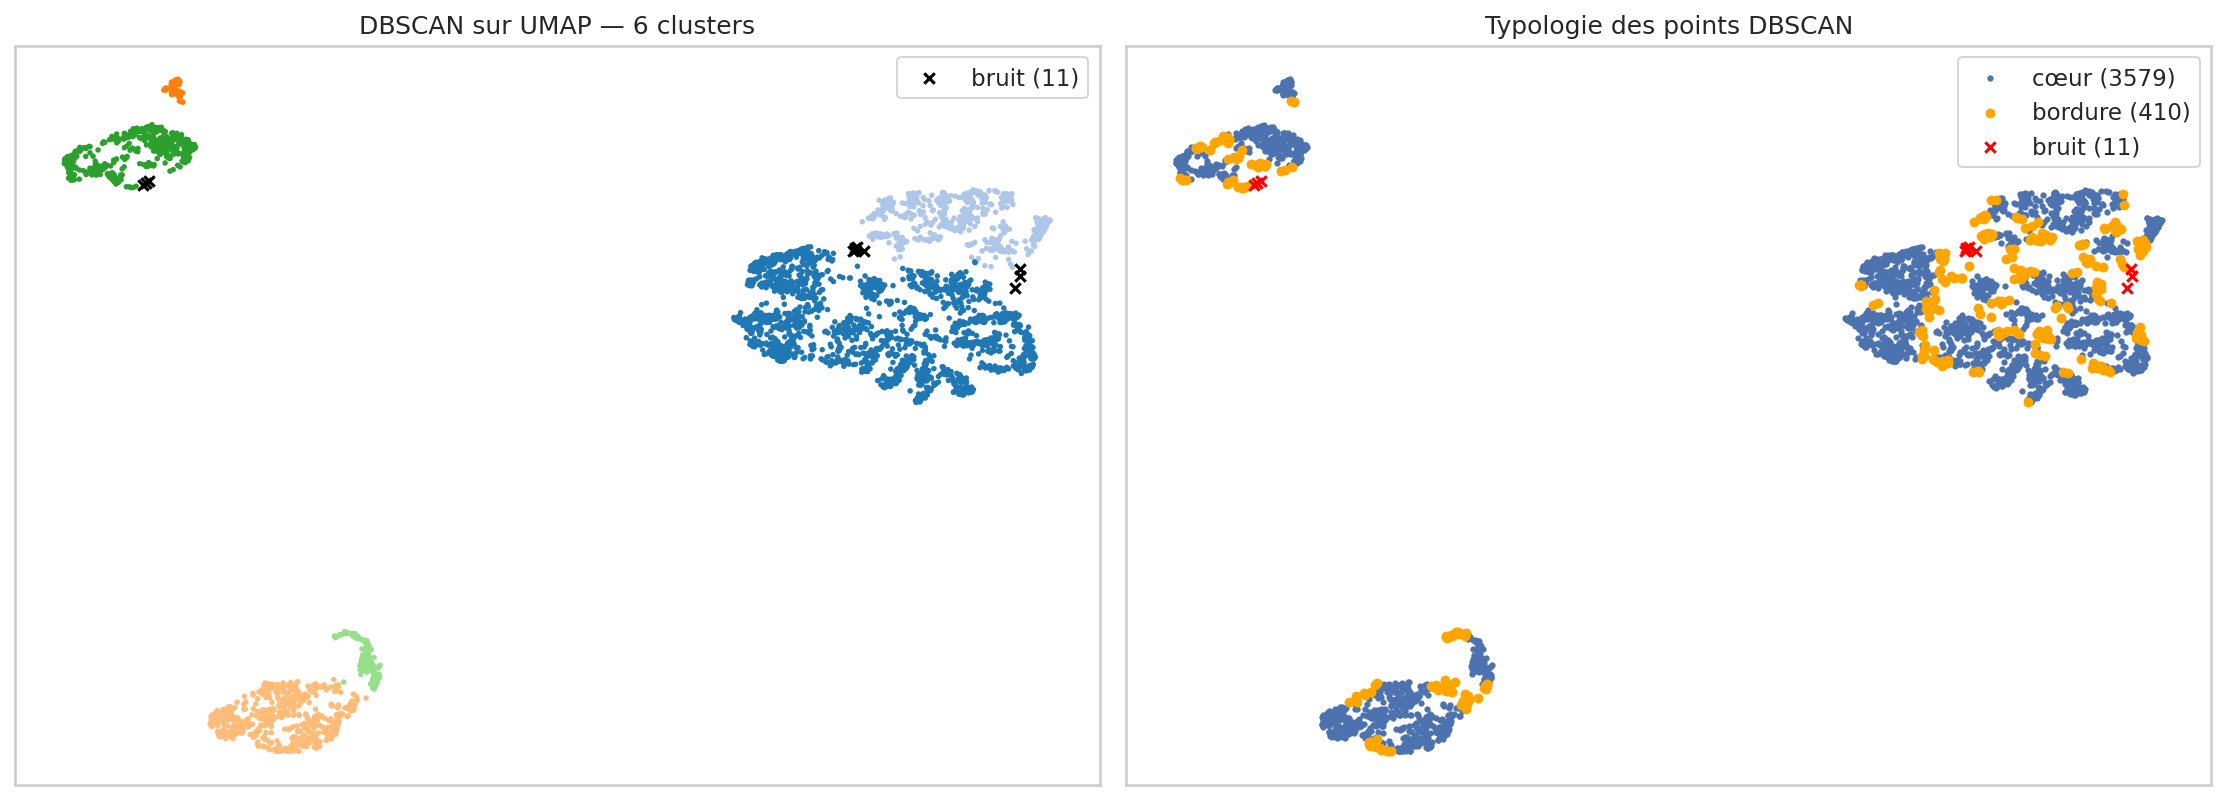
\includegraphics[width=.9\linewidth]{j3_dbscan_umap.png}
\caption{DBSCAN sur UMAP : clusters, points cœur, de bordure et bruit.}\label{fig:db}
\end{figure}

\subsection{Limites de K-means}
Sur un jeu contrôlé (deux lunes et 25 points isolés), K-means coupe linéairement les lunes et absorbe les isolés, alors que DBSCAN suit les formes non convexes et étiquette le bruit. Sur UMAP, K-means scinde ou fusionne arbitrairement les îlots.

DBSCAN a cependant ses propres limites : il dépend d'un seul $\varepsilon$, ce qui pose problème si les densités sont hétérogènes ; il se dégrade en grande dimension ; il n'affecte pas nativement un nouveau client. C'est un excellent outil exploratoire et de détection d'atypiques, moins un outil de segmentation opérationnelle.

%=====================================================================
\section{Validation}\label{sec:valid}
\subsection{Indices internes et externes}
Pour 6 familles × 9 valeurs de $k$ ainsi que DBSCAN, nous avons calculé :
\begin{itemize}
\item les indices internes dans l'espace commun (a) : silhouette, Davies-Bouldin et Dunn (implémentation personnelle), plus la silhouette Gower ;
\item les indices externes par rapport à \texttt{y} : ARI, NMI, homogénéité, complétude, V-mesure.
\end{itemize}

\begin{figure}[H]\centering
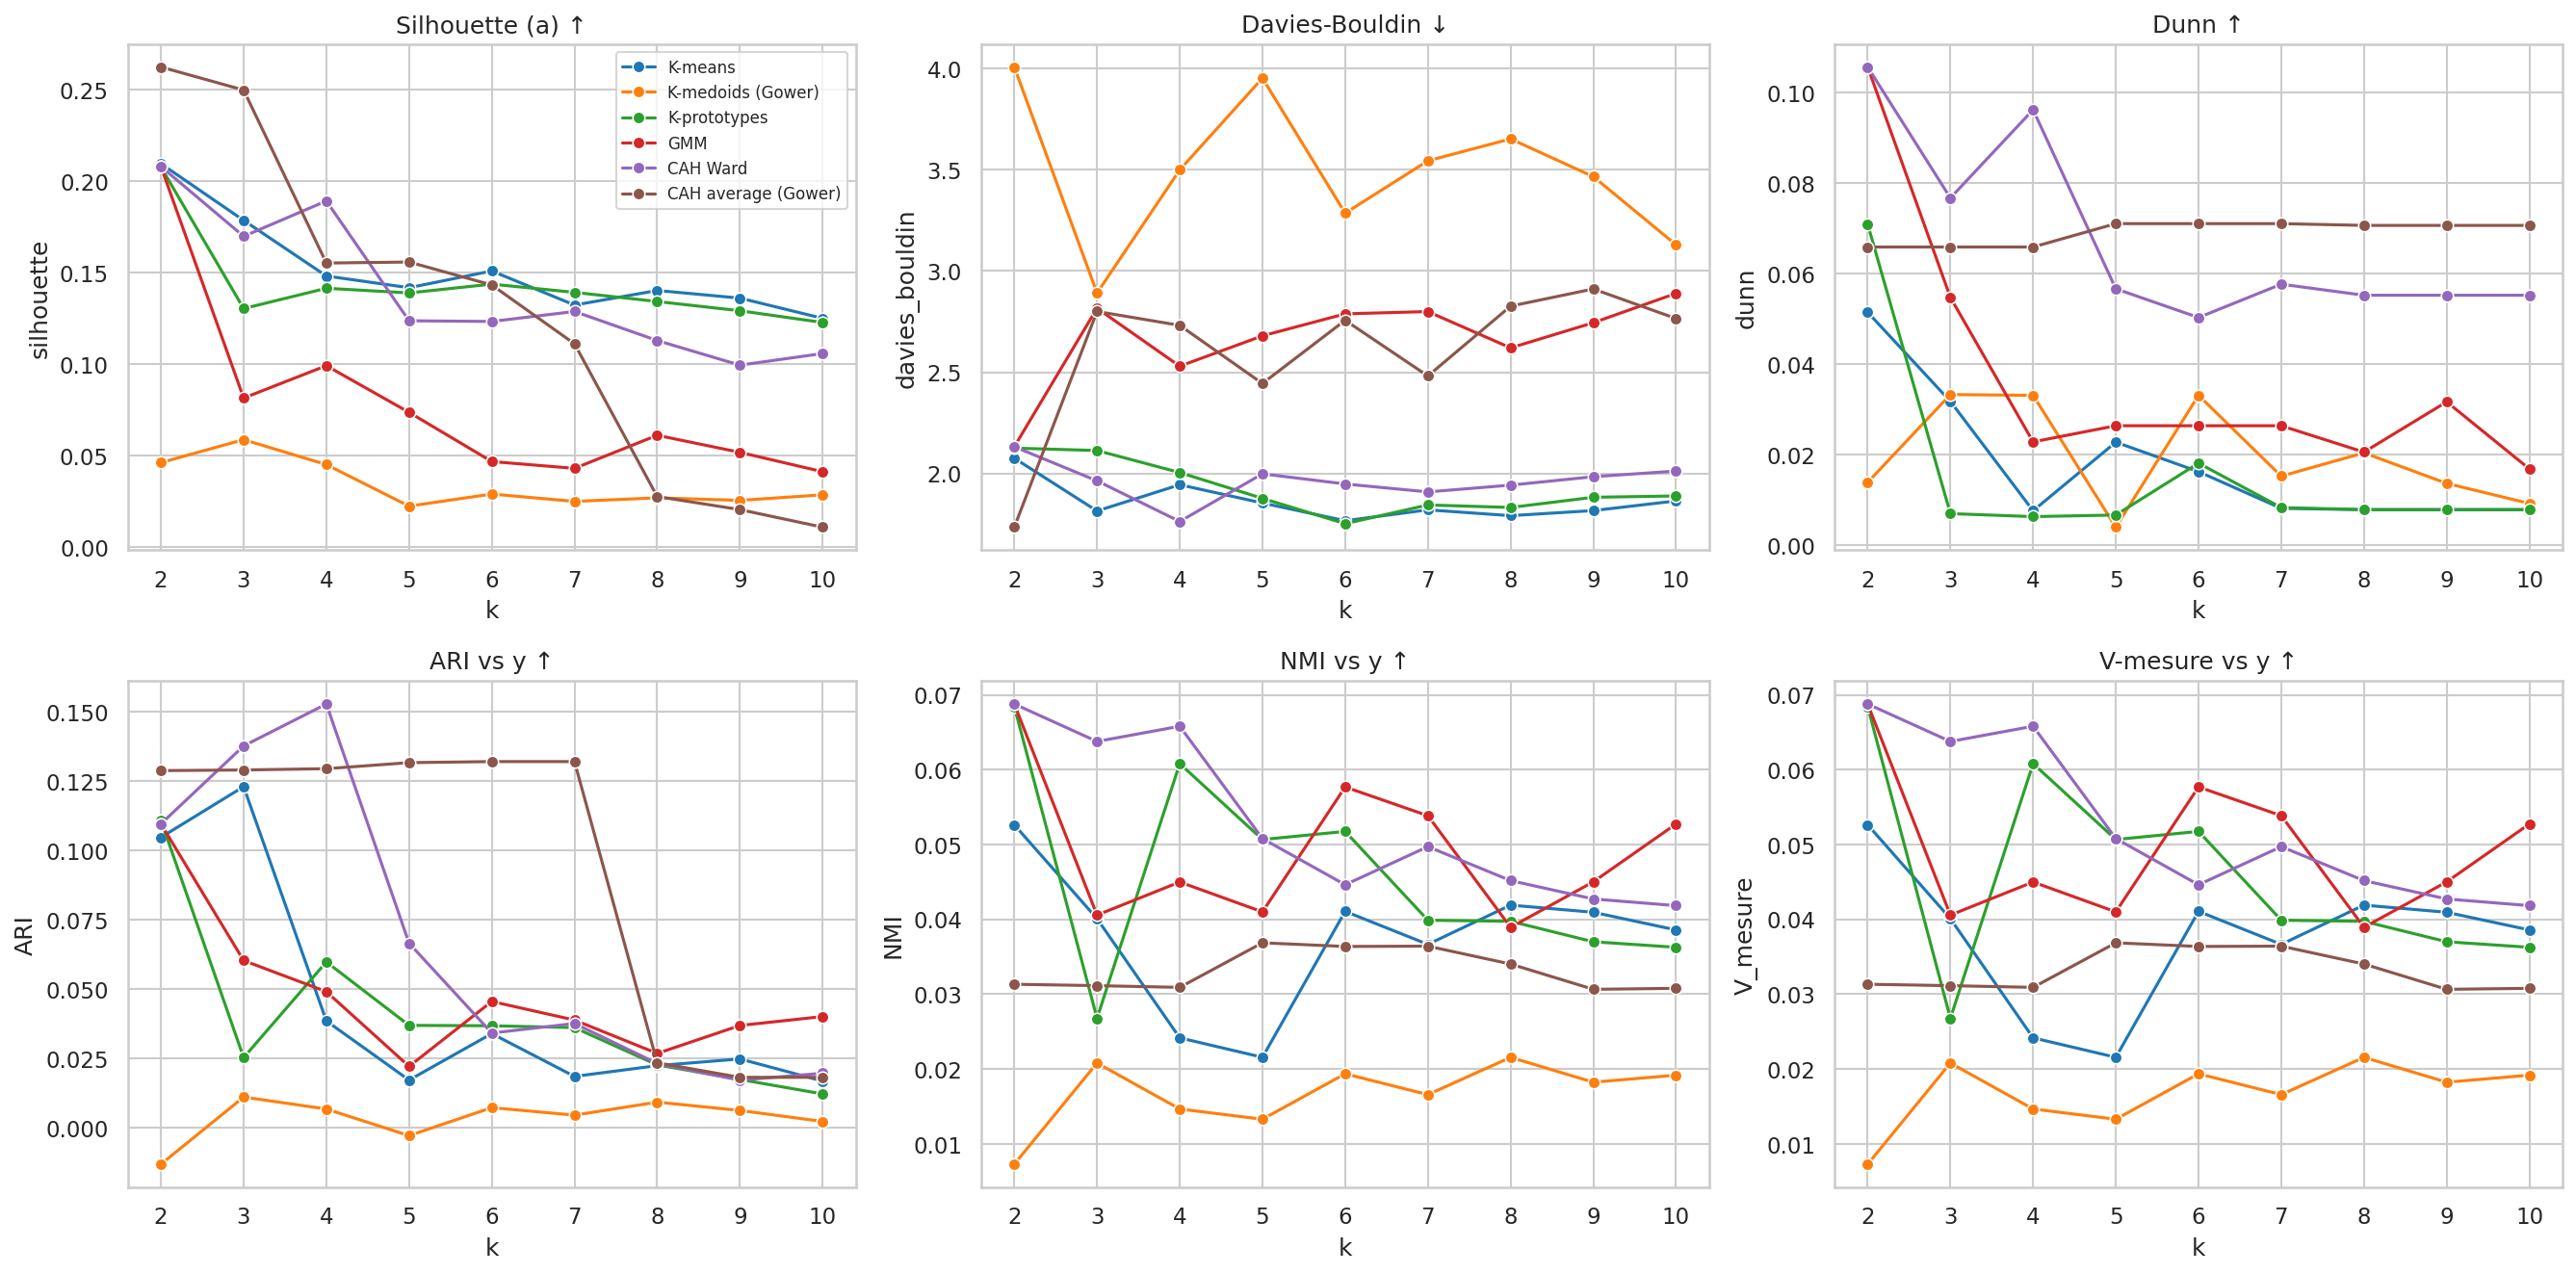
\includegraphics[width=\linewidth]{j4_indices_par_k.png}
\caption{Indices internes et externes en fonction de $k$.}
\end{figure}

La silhouette décroît avec $k$ (structure grossière dominante) et reste modeste (< 0,25), ce qui est attendu pour des données mixtes aux groupes recouvrants. L'indice de Dunn est très faible partout : il dépend d'un seul couple min/max et est très sensible aux atypiques. Davies-Bouldin est le plus discriminant.

Les indices externes sont faibles (ARI < 0,16), ce qui est \textbf{souhaitable} : une segmentation décrit des profils et ne cherche pas à reproduire une décision binaire déséquilibrée. On s'intéresse plutôt à l'\emph{homogénéité}, qui traduit des segments aux taux de souscription contrastés.

\subsection{Stabilité}
K-means a été relancé avec 20 graines (\texttt{n\_init}=1, 190 paires) et sur 20 rééchantillonnages bootstrap de la population, chaque modèle affectant ensuite toute la population.
\begin{itemize}
\item La sensibilité à l'initialisation est réelle (ARI moyen 0,60–0,93), d'où \texttt{n\_init} ≥ 10.
\item En bootstrap, $k=2$, 4 et 5 sont stables (ARI ≥ 0,94) ; $k=3$ (0,72 ± 0,28) et $k\geq9$ le sont moins.
\end{itemize}

\subsection{Sélection de la solution}
Nous avons retenu cinq critères : actionnabilité (3 à 6 segments, aucun < 5\,\%), qualité interne, stabilité, homogénéité vis-à-vis de \texttt{y} et déployabilité. Un score par rangs (silhouette, Davies-Bouldin, V-mesure) place la \textbf{CAH Ward à $k=4$ en tête sur les trois critères}. Comme la CAH ne sait ni affecter un nouveau client ni passer à l'échelle, nous avons adopté une \textbf{classification mixte} : les 4 barycentres Ward initialisent un K-means sur les 41\,176 clients.

\begin{table}[H]\centering\small
\begin{tabular}{lcccccc}\toprule
Méthode & $k$ & Silh. (a) & DB & Silh. Gower & ARI & V-mesure\\\midrule
CAH Ward & 4 & 0,189 & 1,76 & 0,168 & 0,153 & 0,066\\
K-means & 6 & 0,151 & 1,77 & 0,119 & 0,034 & 0,041\\
K-prototypes & 5 & 0,139 & 1,88 & 0,102 & 0,037 & 0,051\\
GMM & 4 & 0,099 & 2,53 & 0,169 & 0,049 & 0,045\\
K-medoids (Gower) & 3 & 0,059 & 2,89 & 0,158 & 0,011 & 0,021\\
DBSCAN (UMAP) & 6 & 0,104 & 2,25 & 0,158 & 0,072 & 0,051\\
DBSCAN (PCA) & 3 & 0,121 & 2,22 & 0,149 & 0,160 & 0,055\\\midrule
\textbf{Ward + K-means (retenue)} & \textbf{4} & \textbf{0,192} & \textbf{1,69} & \textbf{0,174} & \textbf{0,151} & \textbf{0,062}\\\bottomrule
\end{tabular}
\caption{Synthèse des indices (meilleure solution admissible par famille, échantillon $n=4\,000$).}\label{tab:synth}
\end{table}

La consolidation reproduit fidèlement Ward (ARI 0,98 sur l'échantillon) et améliore silhouette et Davies-Bouldin. Elle est \textbf{extrêmement stable} au rééchantillonnage une fois les centres fixés (ARI bootstrap 0,999).

\emph{Limite} : la chaîne complète, avec une CAH refaite sur chaque bootstrap, est moins stable (ARI 0,72 ± 0,23), car la CAH coupe parfois différemment les petits groupes. Il faut donc figer les centres de référence et les ré-estimer périodiquement. Enfin, K-means standard à $k=4$ atteint une inertie plus faible (234\,094 contre 243\,332), mais avec une moins bonne séparation (silhouette 0,148).

%=====================================================================
\section{Interprétation et recommandations}\label{sec:interp}
\begin{table}[H]\centering\small
\begin{tabular}{lrrrrrr}\toprule
 & \textcolor{s1}{\textbf{S1}} & \textcolor{s2}{\textbf{S2}} & \textcolor{s3}{\textbf{S3}} & \textcolor{s4}{\textbf{S4}} & Ensemble\\\midrule
Clients (\%) & 65,4 & 17,0 & 6,2 & 11,4 & 100\\
Âge moyen & 40,2 & 37,7 & 47,0 & 38,9 & 40,0\\
Appels (campaign) & 2,83 & 2,23 & 1,82 & 2,00 & 2,57\\
Contacts antérieurs & 0,00 & 0,00 & 0,41 & 1,30 & 0,17\\
Euribor 3 mois & 4,84 & 1,30 & 0,79 & 1,64 & 3,62\\
Confiance des ménages & −39,4 & −45,9 & −31,5 & −43,8 & −40,5\\
Mobile (\%) & 49 & 90 & 87 & 93 & 63\\
Défaut non déclaré (\%) & 26 & 13 & 3 & 12 & 21\\
\textbf{Taux de souscription (\%)} & \textbf{4,9} & \textbf{17,3} & \textbf{42,5} & \textbf{22,0} & \textbf{11,3}\\
Lift & ×0,43 & ×1,54 & ×3,77 & ×1,95 & 1\\\bottomrule
\end{tabular}
\caption{Profils moyens des quatre segments (population complète).}\label{tab:prof}
\end{table}

\begin{figure}[H]\centering
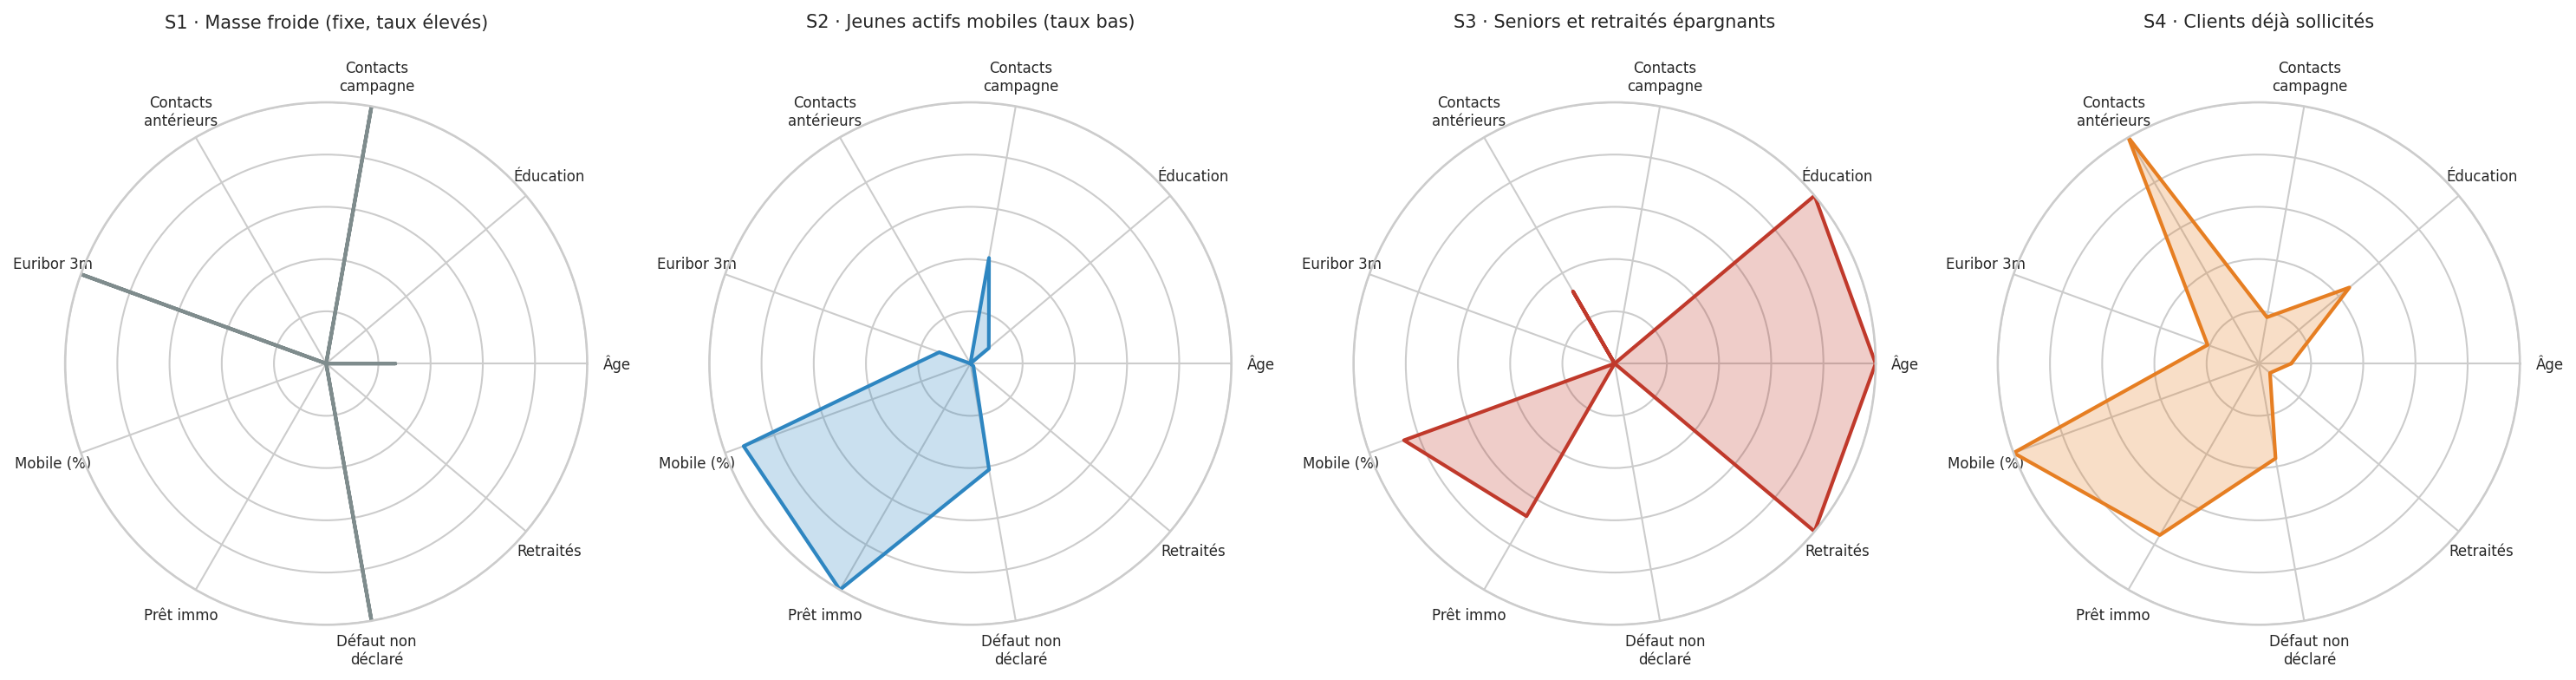
\includegraphics[width=\linewidth]{j5_radars.png}
\caption{Radar charts (moyennes ramenées entre le segment le plus bas et le plus haut).}
\end{figure}

\begin{figure}[H]\centering
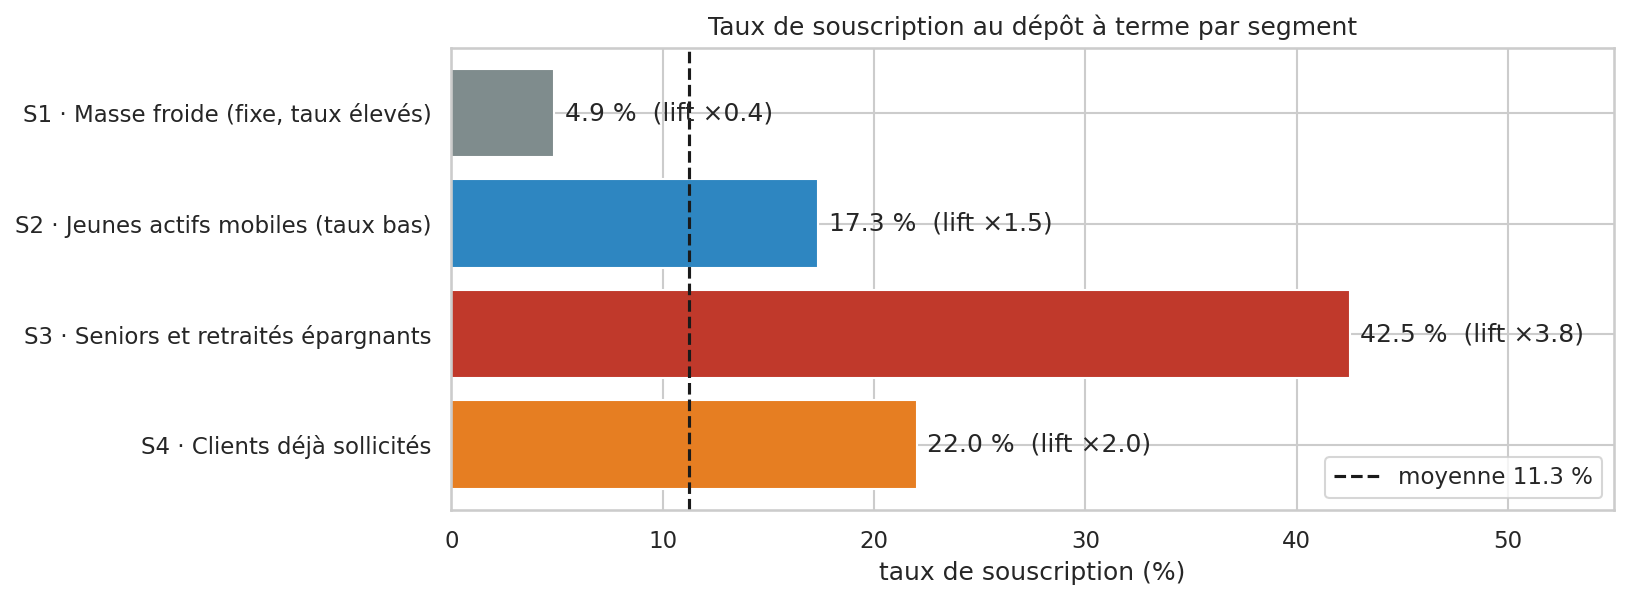
\includegraphics[width=.75\linewidth]{j5_taux_souscription.png}
\caption{Taux de souscription par segment (la cible n'intervient qu'\emph{a posteriori}).}
\end{figure}

\paragraph{\textcolor{s1}{S1 — Masse froide (fixe, taux élevés), 65\,\%}.} Ces clients n'ont jamais été contactés auparavant et ont été joints pour moitié sur ligne fixe, en période de taux élevés. Ils subissent la plus forte pression d'appel (2,8 appels) pour seulement 4,9\,\% de souscription. \textbf{Recommandation} : plafonner à 2 appels et basculer sur des canaux à bas coût (SMS, e-mail, application). L'appel conseiller ne se déclenche qu'après un signal d'intérêt (clic, simulation). Il faut aussi compléter les données manquantes.

\paragraph{\textcolor{s2}{S2 — Jeunes actifs mobiles, 17\,\%}.} 38 ans en moyenne, 36\,\% de célibataires, joignables sur mobile, contactés en période de taux bas et de forte inquiétude économique (17,3\,\%). \textbf{Recommandation} : campagne \emph{mobile-first} (SMS + rappel) proposant un dépôt à terme court et accessible (petit ticket, sortie anticipée). L'argumentaire porte sur l'épargne de précaution, avec un parcours de souscription 100\,\% digital.

\paragraph{\textcolor{s3}{S3 — Seniors et retraités épargnants, 6\,\%}.} 47 ans, 21\,\% de retraités, presque aucun défaut non déclaré, une partie déjà convertie par le passé : 42,5\,\% de souscription (lift ×3,8). \textbf{Recommandation} : segment prioritaire, confié à des conseillers dédiés. On propose des dépôts longs à taux garanti mettant en avant la sécurité du capital, avec rendez-vous en agence ; un seul appel suffit.

\paragraph{\textcolor{s4}{S4 — Clients déjà sollicités, 11\,\%}.} Tous ont été contactés lors d'une campagne précédente (80\,\% d'échecs, 20\,\% de succès) ; 22\,\% souscrivent. \textbf{Recommandation} : recontacter en priorité les anciens souscripteurs avec une offre de renouvellement. Pour les échecs, il faut changer d'offre et d'argumentaire plutôt que répéter le même appel, en espaçant les relances.

\paragraph{Lecture transversale.} S2, S3 et S4 représentent 35\,\% des clients mais \textbf{72\,\% des souscripteurs}. Concentrer les appels conseillers sur ces segments et traiter S1 par des canaux à bas coût réduirait fortement le volume d'appels pour un nombre de souscriptions comparable.

L'analyse temporelle \emph{a posteriori} (figure~\ref{fig:temps}) montre un \textbf{effet de période massif} : S1 regroupe la quasi-totalité des appels de 2008, et S3 n'émerge qu'en 2010. Une partie de la segmentation reflète donc le contexte de taux autant que le client. C'est actionnable (choisir \emph{quand} appeler), mais cela impose une mise à jour régulière.

\begin{figure}[H]\centering
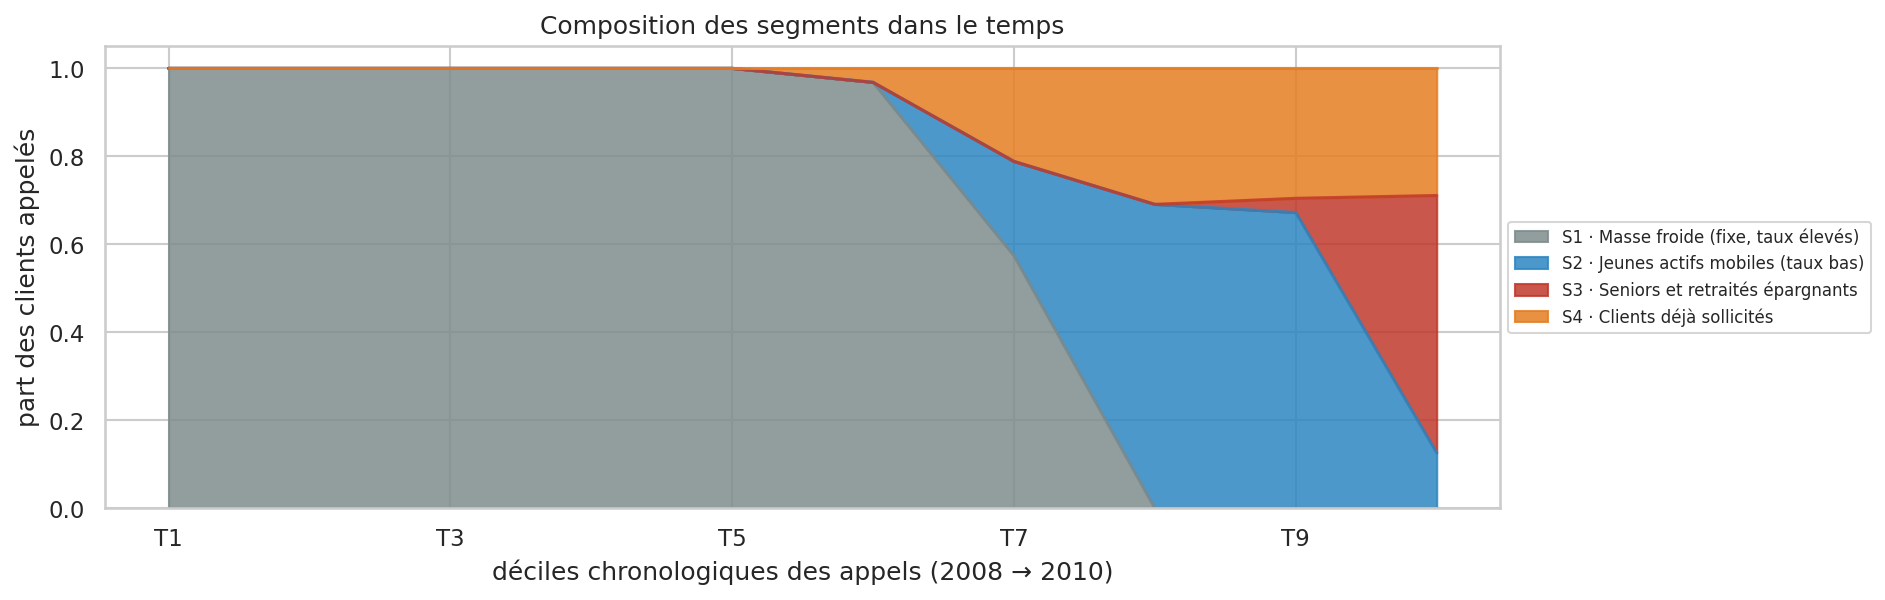
\includegraphics[width=.85\linewidth]{j5_segments_temps.png}
\caption{Composition des segments selon les déciles chronologiques des appels.}\label{fig:temps}
\end{figure}

%=====================================================================
\section{Extensions (bonus)}\label{sec:bonus}
\subsection{Détection d'anomalies}
Isolation Forest (300 arbres, contamination 1\,\%) isole \textbf{411 clients atypiques}. Ce sont des clients plus âgés (51 ans), au long historique (2 contacts antérieurs contre 0,15 ; 64\,\% d'anciens succès), souvent retraités ou étudiants (47\,\% contre 6\,\%). Leur taux de souscription atteint \textbf{54\,\%}.

Ce ne sont donc pas des erreurs mais des niches à très forte valeur, logées dans S3 et S4, qui relèvent d'un suivi individuel. Le bruit DBSCAN en PCA a un score d'anomalie moyen supérieur à celui de l'échantillon (0,55 contre 0,46) et recouvre 21\,\% des atypiques Isolation Forest.

\subsection{Sélection de caractéristiques}
Quatre jeux de variables ont été comparés, chacun évalué par K-means à $k=4$ sur l'échantillon (tableau~\ref{tab:fs}) :
\begin{itemize}
\item un filtre de variance sur les indicatrices (seuil 0,03), qui retire 3 petits métiers ;
\item un filtre de corrélation ($|r|>0{,}7$), qui retire 2 indicatrices redondantes ;
\item un \emph{wrapper} par sélection avant pas à pas maximisant la silhouette ;
\item une variante « profil pur » sans indicateurs macro-économiques.
\end{itemize}

\begin{table}[H]\centering\small
\begin{tabular}{lcccc}\toprule
Jeu de variables & Colonnes & Silhouette & V-mesure ($y$) & V de Cramér (période)\\\midrule
Toutes & 27 & 0,148 & 0,024 & 0,54\\
Filtre variance & 24 & 0,150 & 0,024 & 0,54\\
Filtre corrélation & 25 & 0,149 & 0,024 & 0,54\\
Wrapper (6 variables) & 8 & 0,561 & 0,060 & 0,57\\
Profil pur (sans macro) & 25 & 0,156 & 0,015 & 0,31\\\bottomrule
\end{tabular}
\caption{Comparaison des méthodes de sélection de variables.}\label{tab:fs}
\end{table}

Le wrapper illustre son biais : \texttt{housing} + \texttt{loan} seuls donnent une silhouette de 1,0, avec 4 combinaisons parfaites mais sans intérêt métier. Le critère s'auto-justifie et doit être validé par l'interprétabilité.

La variante « profil pur » divise par près de deux la dépendance à la période, au prix d'un pouvoir discriminant plus faible sur \texttt{y}. C'est la preuve que le contexte de taux explique une large part de la souscription.

\subsection{Application Streamlit}
\texttt{app/streamlit\_app.py} affecte un nouveau client à un segment à partir d'un formulaire. L'application réutilise exactement le pipeline de prétraitement et les centroïdes finaux ; son accord avec les étiquettes du modèle est de 100\,\% sur 300 clients tirés au hasard. Elle affiche la fiche du segment, la recommandation, les distances aux centres et la position du client en projection PCA. Elle permet aussi l'affectation par lot d'un fichier CSV avec téléchargement du résultat.

\subsection{Second jeu : Online Retail (RFM)}
Après nettoyage (suppression des clients anonymes, des factures d'annulation et des quantités ou prix négatifs), il reste 4\,338 clients décrits par la récence, la fréquence et le montant (transformation $\log(1+x)$ puis z-score). K-means à $k=4$ donne une silhouette de 0,34, bien plus nette que sur Bank Marketing, et une forte stabilité (ARI bootstrap 0,91).

Les \textbf{Champions} (16\,\% des clients) génèrent \textbf{65\,\% du chiffre d'affaires} ; viennent ensuite les Réguliers à relancer (27\,\% des clients, 24\,\% du CA), les Nouveaux clients et les Perdus (37\,\% des clients, 6\,\% du CA). La segmentation par quintiles RFM est cohérente mais différente (ARI 0,32) : ses seuils sont arbitraires, alors que le clustering découvre les frontières dans les données.

%=====================================================================
\section{Discussion et conclusion}
\paragraph{Apports.} La démarche complète montre trois points :
\begin{itemize}
\item Le choix de la \emph{représentation} et de la \emph{distance} pèse autant que celui de l'algorithme : la standardisation change 68\,\% des plus proches voisins, et Gower et l'euclidienne aboutissent à des partitions différentes.
\item Les indices internes doivent être lus ensemble et avec des contraintes métier : la silhouette maximale (lien single, $k=2$) correspond aux pires segmentations.
\item Une classification mixte Ward + K-means combine la qualité de la CAH et la déployabilité de K-means.
\end{itemize}

\paragraph{Limites.}
\begin{itemize}
\item Les silhouettes restent modestes : les groupes se recouvrent.
\item La segmentation est fortement liée à la période d'appel via \texttt{euribor3m}.
\item La chaîne CAH → K-means est sensible au rééchantillonnage.
\item Les données datent de 2008–2010 et concernent un seul établissement.
\end{itemize}

\paragraph{Perspectives.} Plusieurs pistes prolongent ce travail :
\begin{itemize}
\item une double segmentation, avec un profil client pur pour le CRM et une segmentation enrichie du contexte pour le pilotage des campagnes ;
\item des distances apprises (encodage des métiers par similarité) ;
\item un suivi de la dérive des segments dans le temps ;
\item un test A/B des recommandations sur une campagne réelle.
\end{itemize}

\paragraph{Conclusion.} Quatre segments interprétables et stables ont été identifiés, avec des taux de souscription allant de 4,9\,\% à 42,5\,\%. Ils débouchent sur des actions marketing concrètes et un outil d'affectation opérationnel.

\vspace{.5cm}
\noindent\textbf{Références.} Moro S., Cortez P., Rita P. (2014). \textit{A data-driven approach to predict the success of bank telemarketing}. Decision Support Systems, 62, 22–31. — Gower J.C. (1971). \textit{A general coefficient of similarity and some of its properties}. Biometrics, 27(4). — Huang Z. (1998). \textit{Extensions to the k-means algorithm for clustering large data sets with categorical values}. DMKD, 2(3). — Ester M. et al. (1996). \textit{A density-based algorithm for discovering clusters}. KDD. — Liu F.T., Ting K.M., Zhou Z.-H. (2008). \textit{Isolation Forest}. ICDM. — McInnes L., Healy J. (2018). \textit{UMAP}. arXiv:1802.03426. — Chen D., Sain S.L., Guo K. (2012). Online Retail dataset, UCI.

\end{document}
